\newpage
\section{Les types de verrouillages\cite{butenhof}}

Il existe deux types de verrous sous Linux : les \textit{Advisory locks} (verrous consultatifs) et les \textit{Mandatory locks} (verrous obligatoires).

\subsection{Visualiser tous les verrous d'un système Linux}

Pour visualiser tous les verrous actifs d'un système Linux, on peut utiliser la commande \texttt{lslocks} ou consulter le fichier \texttt{/proc/locks} qui fournit des informations détaillées sur les verrous actuellement détenus par les processus. À noter que j'ai remarqué que la commande \texttt{lslocks} se base sur le fichier \texttt{/proc/locks} afin de construire son output.

\subsection{Advisory Locks}

Les Advisory locks (consultatifs) permettent aux processus de demander un verrou sur un fichier, sans empêcher d'autres processus d'accéder ou de modifier le fichier. Ils sont particulièrement utiles lorsque plusieurs processus doivent accéder à un fichier, mais chacun doit garantir un accès exclusif à une section particulière du fichier. 

Il ne fonctionnera que si les processus demandent explicitement des verrous. Si un des processus n'a pas connaissance d'un verrou, alors il sera ignoré. Les 2 processus qui veulent un accès en concurrence doivent essayer d’acquérir le verrou pour accéder au fichier. Ce verrou n’est ni donné par l’OS, ni par le File System. Il est donc très important de comprendre que les processus doivent être coopératifs pour que le verrou soit mis en oeuvre.
\newline
Pour bien imprégner cette notion, voici un exemple : 

Dans un premier temps, nous avons un premier \texttt{process (A)} qui viendra verrouiller un fichier contenant une valeur (balance) et puis soustraire à cette valeur, son argument.

Ensuite, une second \texttt{process (B)} viendra également modifier la valeur du fichier balance en y additionnant la valeur de son argument mais sans employer aucun verrou.

En lançant à la suite des autres les process A et B, avec une balance initialisée avec la valeur 100. Le process B n'étant pas coopératif, il n'attendra pas A avant d'écrire dans la balance, le verrou demandé par A est donc ignoré et la valeur finale de B est éronée (180 au lieu de 160) car B écrasera simplement la valeur définie par A afin d'écrire la sienne.
\newline

Voici un détail de l'exécution : 
\begin{verbatim}
Le process A lit la valeur actuelle du fichier (100) .
Le process B lit maintenant le même fichier et obtient le solde actuel (100).
Le process A calcule 100 - 20 et enregistre le résultat 80 dans le fichier.
Le process B ne sait pas que le solde a été mis à jour depuis sa dernière lecture.
\end{verbatim}

En conséquence, B utilisera toujours la valeur obsolète 100 pour calculer 100 + 80 et écrire le résultat 180 dans le fichier \texttt{balance} au lieu de la valeur attendue 160.
\newline

Imaginons maintenant un process B qui sera coopératif avec A et qui fera une demande d'accès pour écrire dans la balance. Cette fois-ci, lorsque l'on exécutera les 2 process un à la suite de l'autre, on observa que le process B attendra d'abord que A libère son accès avant de lui-même commencer à écrire dans le fichier protégé. Dans ce cas, le résulat final est bel et bien celui attendu.
\newline

Voici un détail de l'exécution : 
\begin{verbatim}
Le process A active son verrou sur le fichier
Le process B doit attendre que le processus A libère le verrou.
Le process A calcule 100 - 20 et écrit 80 dans le fichier.
Le process A libère le verrou.
Le process B acquiert maintenant un verrou et lit le fichier
Le process B obtient ainsi la valeur mise à jour : 80.
Le process B démarre sa logique et écrit le résultat 160 (80 + 80) dans le fichier.
Le process B libère le verrou
\end{verbatim}

Cela démontre donc que les avisory locks reposent exclusivement sur la coopérativité des process.

Dans la théorie, c'est simple, mais cela ne nous explique pas comment est-ce interprété par le noyau. Reprenons donc cet exemple et voyons comment le mettre en pratique. 
\newline

\begin{itemize}
    \item Le script \texttt{updated\_balance.sh} gère la logique de mise à jour du solde pour les deux process.
    \item Les 2 process A et B utilisent donc \texttt{updated\_balance.sh} pour leur logique.
    \item Quant aux verrous, ils sont donnés aux process A et B via :
    \begin{lstlisting}
    flock --verbose balance.dat ./updated_balance.sh
    \end{lstlisting}
    \item L'argument \texttt{balance.dat} de la commande est le fichier sur lequel doit être appliqué le verrou.
    \item L'argument \texttt{./updated\_balance.sh} de la commande est la commande à exécuter une fois le verrou activé.
    \item Nous pouvons vérifier les informations de verrouillage via la commande \texttt{lslocks} (on peut rajouter \texttt{| grep 'balance'} pour n'avoir que celui qui nous intéresse).
\end{itemize}
\begin{figure}[h]
    \centering
    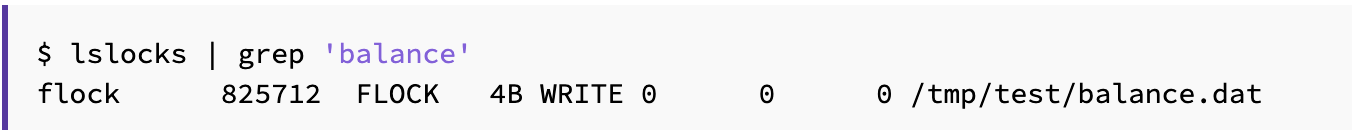
\includegraphics[width=0.8\textwidth]{img/lslocks-balance.png}
    \caption{Capture d'écran de la commande \texttt{lslocks} avec \texttt{balance}}
    \label{fig:lslocks-balance}
\end{figure}
Selon cet output, on peut en déduire que le verrou a été appliqué avec la commande \texttt{flock}, la taille du verrou est de 4B et en mode écriture et qu'il a été appliqué sur le fichier /tmp/test/balance.dat via le process pid=825712
\newline

\textbf{Remarque:} Une démo de ce script est disponible dans l'archive tar que vous pouvez consulter. De plus, le code et les scripts dans entièreté se trouvent sur ce git\cite{git} afin que vous puissiez tester cette expérience dans votre environnement et manipuler les codes à votre guise.
\newline

\subsection{Mandatory Locks}

Jusqu'ici, on pourrait très bien se débrouiller avec des sémahpores. Rien de très révolutionnaire. Mais voyons maintenant l'une des plus grosse différences.
\newline

Les Mandatory locks (verrous obligatoires) sont définis par le noyau et ne peuvent pas être annulés par les processus. La fonction \texttt{fcntl()} est également utilisée pour définir des verrous obligatoires sur les fichiers.

Il ne requiert aucune coopération entre les processus. Si un mandatory locking est activé sur un fichier, c’est l’OS qui prend en charge le verrou et qui avertira les process. Le principe de "celui qui ne joue pas le jeu n'est pas bloqué" n'est donc pas d'actualité.
\newline

Si un processus essaie d'effectuer un accès sur la région d'un fichier qui a un verrou obligatoire, le résultat dépendra de l'attribut \texttt{O\_NONBLOCK} pour son description de fichier. Si l'attribut \texttt{O\_NONBLOCK} n'est pas activé, l'appel système bloquera jusqu'à ce que le verrou soit liberé. Si l'attribut \texttt{O\_NONBLOCK} est activé, l'appel système échouera.
\newline

Dans un environnement où plusieurs utilisateurs accèdent à un fichier, le mandatory locking assure un accès exclusif à un enregistrement. Sans cela, des conflits de mise à jour simultanée pourraient conduire à des pertes de données. Avec le mandatory locking, un utilisateur obtient un verrou exclusif sur l'enregistrement, empêchant d'autres utilisateurs d'y accéder tant que le verrou est détenu. Ce verrou est indépendant des droits du fichier, ni du créateur car le verrou est appliqué directement sur le système de fichier.
\newline

Ils ne sont généralement pas activés par défaut sur les systèmes d'exploitation car il ajoute une complexité supplémentaires aux systèmes de fichiers qui n'en n'ont pas pour la plupart du temps pas besoin.
\newline

Voici les étapes pour activer le mandatory locking sur Linux et leur effet sur le noyau :

\begin{itemize}
  \item Le système de fichiers (FS) doit être monté avec l'option \texttt{mand} :
        \begin{verbatim}
        mount -o mand FILESYSTEM MOUNT_POINT
        \end{verbatim}
    Cela permet d'indiquer au noyau d'activer le support du mandatory locking pour ce système de fichiers particulier. \newline
    
  \item Il faut activer le bit \texttt{set-group-ID} et désactiver le bit \texttt{group-execute} pour tous les fichiers que l'on veut bloquer :
        \begin{verbatim}
        chmod g+s, g-x FILE
        \end{verbatim}
        \texttt{g+s} active le bit set-group-ID sur le fichier. Cela signifie que lorsque le fichier est exécuté, il hérite du groupe du répertoire parent, assurant que tous les membres du groupe ont des droits cohérents.
        \newline
        \texttt{g-x} désactive le bit group-execute sur le fichier, ce qui empêche les membres du groupe d'exécuter le fichier. C'est nécessaire pour ne pas que l'exécution du fichier n'interfére avec le mécanisme de verrouillage.
\end{itemize}

\subsection{L'output de lslocks}
En observant l'output complet de \texttt{lslocks} dans mon terminal, j'ai remarqué qu'il y avait plusieurs locks actifs sur mon système, je me suis donc penché dessus et j'ai observé qu'ils se rapportaient, pour une majorité, à un process en cours d'utilisation. Par exemple, lorsque j'utilise Firefox, le process apporte son lot de verrous. En effet, ils ont tous le même pid et le nom des fichiers verrouillés sont explicites. J'ai fait le test de terminer le process et les locks sont désactivés. Pour mieux comprendre à quoi servent ces verrous j'ai analysé les fichiers sur lesquels ils ont été posés ; les fichiers verrouillés sont en majorité des bases de données locales relatives entre autre aux favoris, aux cookies et d'autres. Les verrous sont de type \texttt{firefox} et qu'ils ont donc leur propre verrou et de type POSIX.

Voici un output concernant les locks de mon systèmes, dont ceux de Mozilla (j'ai volontairement coupé une partie de l'output non-nécessaire pour cette illustration).
\begin{figure}[ht]
  \centering
  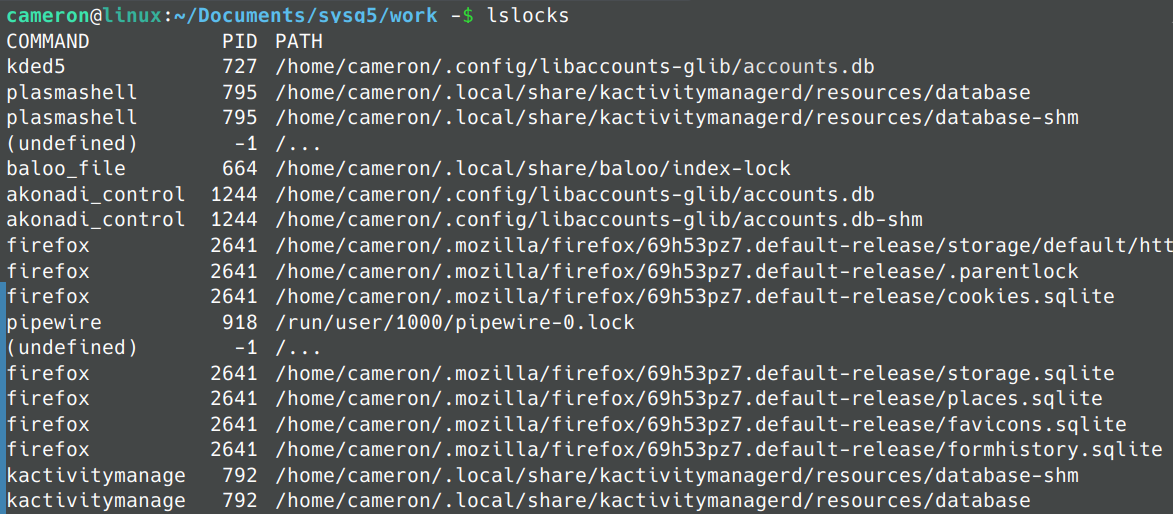
\includegraphics[width=1.0\textwidth, height=8cm]{img/lslock-output.png}
    \caption{Capture d'écran de la commande \texttt{lslocks} avec Mozilla}
    \label{fig:lslocks-mozilla}
\end{figure}
\newline
Je vous invite à faire l'expérience afin de comprendre, sur votre système, quelles sont les potentielles régions critiques.

Pour vous aider à comprendre l'output résultant de la commande, voici les colonnes importantes\cite{ManLslock}
\begin{itemize}
    \item \textbf{COMMAND:} Le nom de la commande ou du processus qui a émis le verrou sur le fichier.
    \item \textbf{PID:} PID du processus qui a émis le verrou.
    \item \textbf{TYPE:} Le type de verrouillage émis sur le fichier (il peut être FLOCK (créé avec flock)  ou  POSIX  (créé  avec fcntl)
    \item \textbf{SIZE:} La taille du verrou en octets.
    \item \textbf{MODE:} Les droits d'accès (lecture, écriture ou * si le process est bloqué).
    \item \textbf{M:} Vaut 1 si verrou obligatoire (mandatory), 0 si requiert coopérativité (1).
    \item \textbf{START:} L'offset à partir duquel le verrou commence dans le fichier.
    \item \textbf{END:} L'offset jusqu'où le verrou s'étend dans le fichier.
    \item \textbf{PATH:} Le chemin complet du fichier verrouillé.
\end{itemize}

Remarque ils n'apparaissent pas tous sur l'image car j'ai réduis les colonnes au minimum. 
